\chapter{Expected Outcomes}
The users can interact with the
system using a GUI. This method will
have higher accuracy in recognition of multiple faces from
a single frame with lower response time.\\    
   	The best model was found to be with FaceNet having testing accuracy exceed 99\%. Other models performed less than this model is due to, FaceNet is a state-of-the-art face recognition system that leverages deep learning techniques, specifically Convolutional Neural Networks (CNNs), to map facial features into a high-dimensional space called an embedding
 Other problem is to detect high variability of human faces in terms of shape, size, pose, expression, illumination, occlusion, and makeup.
FaceNet uses a triplet loss function during training. The loss is computed based on triplets of images: an anchor image of a face, a positive image of the same face (from a different view or under different lighting conditions), and a negative image of a different face.
Other model are MTCNN(Multi-task Cascaded Convolutional Networks)  and CNN(Convolutional Neural Network) is known for its efficiency and accuracy in face detection tasks.

\begin{figure}[h]
\begin{center}
	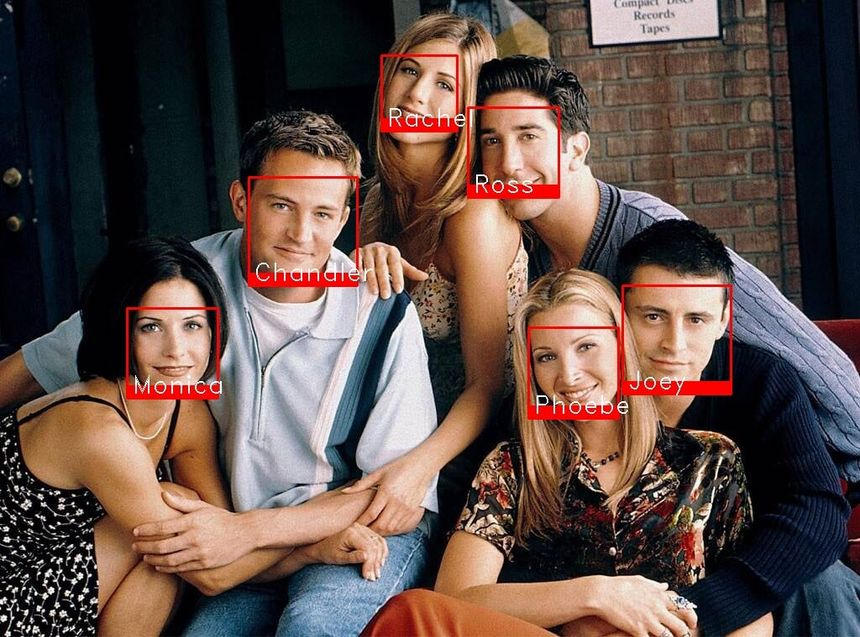
\includegraphics[scale=0.3]{Image/face-recognition-output.jpg}
    \caption{face recognition output}
\end{center}
\end{figure}
\newpage

However, all above models have high accuracy in facial recognition, for face tracking we can integrate tracking algorithm mention above. we like to go for Correlation Filter Tracking which is best for real time tracking with high performance when combine with MTCNN, FaceNet and CNN facial recognition models.
      
\begin{figure}[h]
	\begin{center}
	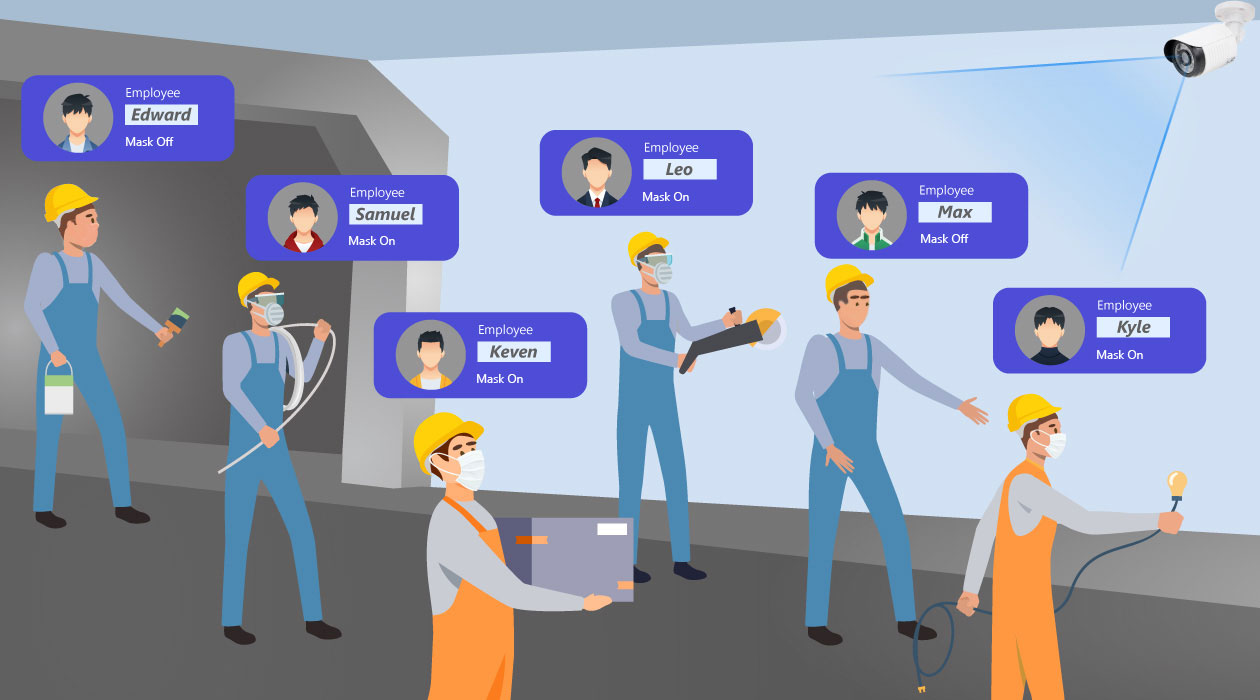
\includegraphics[scale=0.3]{Image/multiPerson-Tracking.jpg}
	\caption{multiPerson-Tracking}
	\end{center}
	
\end{figure}

\section{Conclusion}
The implementation of a Facial Recognition Along With Real-Time Tracking aligns with technological advancements, offering a more accurate and efficient solution for Facial tracking of person. This proposal lays the foundation for a robust system that addresses the current challenges in security surveillance with very high accuracy of recognition and tracking. 
\pagebreak